\chapter{Rappresentazione della scacchiera e dei pezzi} %\label{1cap:spinta_laterale}
% [titolo ridotto se non ci dovesse stare] {titolo completo}
%

\begin{citazione}
    In questo capitolo viene mostrato passo passo un procedimento guida alla realizzazione di un motore scacchistico
\end{citazione}

\newpage

\section{Introduzione} %\label{1sec:scopo}
Il primo passo dello sviluppo di un motore scacchistico è decidere come si vuole rappresentare
la scacchiera , si tratta di una scelta fondamentale,non solo perché in seguito ci permetterà
di testare le funzioni che andremo a implementare, ma anche perché è nella scacchiera che ,generalmente,
viene conservato lo stato generale della partita.\footnote{per stato di una partita si intendono informazioni come
    informazioni su chi ha diritto di muovere, i permessi di arrocco,lo stato della regola delle 50 mosse etc}
Inoltre il tipo di codifica può influenzare la rapidità
e la facilità col quale possiamo accedere alle informazioni sullo stato corrente dei pezzi
e come vedremo in seguito è in grado di influenzare funzioni come la generazione delle mosse.
Non è raro per motori scacchistici particolarmente complessi l'utilizzo di più tipi di board in base
al tipo di informazione da conservare e all'utilizzo che se ne vuole fare.
Per la rappresentazione di una scacchiera sono chiaramente possibili moltissime scelte, di seguito
verranno illustrate alcune tra le più popolari ed utilizzate.

\section{Rappresentazione della scacchiera Pezzocentrica}
Si definisce rappresentazione pezzocentrica, un qualsiasi tipo di rappresentazione della scacchiera che mantiene liste
array o set dei pezzi attualmente presenti sulla scacchiera con annesse le informazioni sulle caselle da essi occupate.
Le rappresentazioni più comuni sono:
\subsubsection{Piece-Lists}
liste o array di ogni pezzo sulla scacchiera,ogni elemento della lista o dell'array associa un pezzo
alla casella che esso occupa .le caratteristiche di ogni pezzo (colore,tipo etc)
possono essere associate all'indice dell'array in cui si trovano o essere presenti in ulteriori array
o liste esterne.

\subsubsection{Bitboards}
Una Bitboard è una struttura dati specifica per i giochi da tavolo,
si tratta in sostanza  di una struttura dati in grado di immagazzinare lo stato di ogni casella della
scacchiera all'interno di una parola \footnote{Una parola è un gruppo di bit di una determinata dimensione che sono gestiti come unità dal set di istruzioni o dall'hardware di un processore} di 64 bit.
Vediamo un esempio pratico, immaginiamo di avere una scacchiera che si trova nello stato di default di inizio
partita:
\begin{figure}
    \centering
    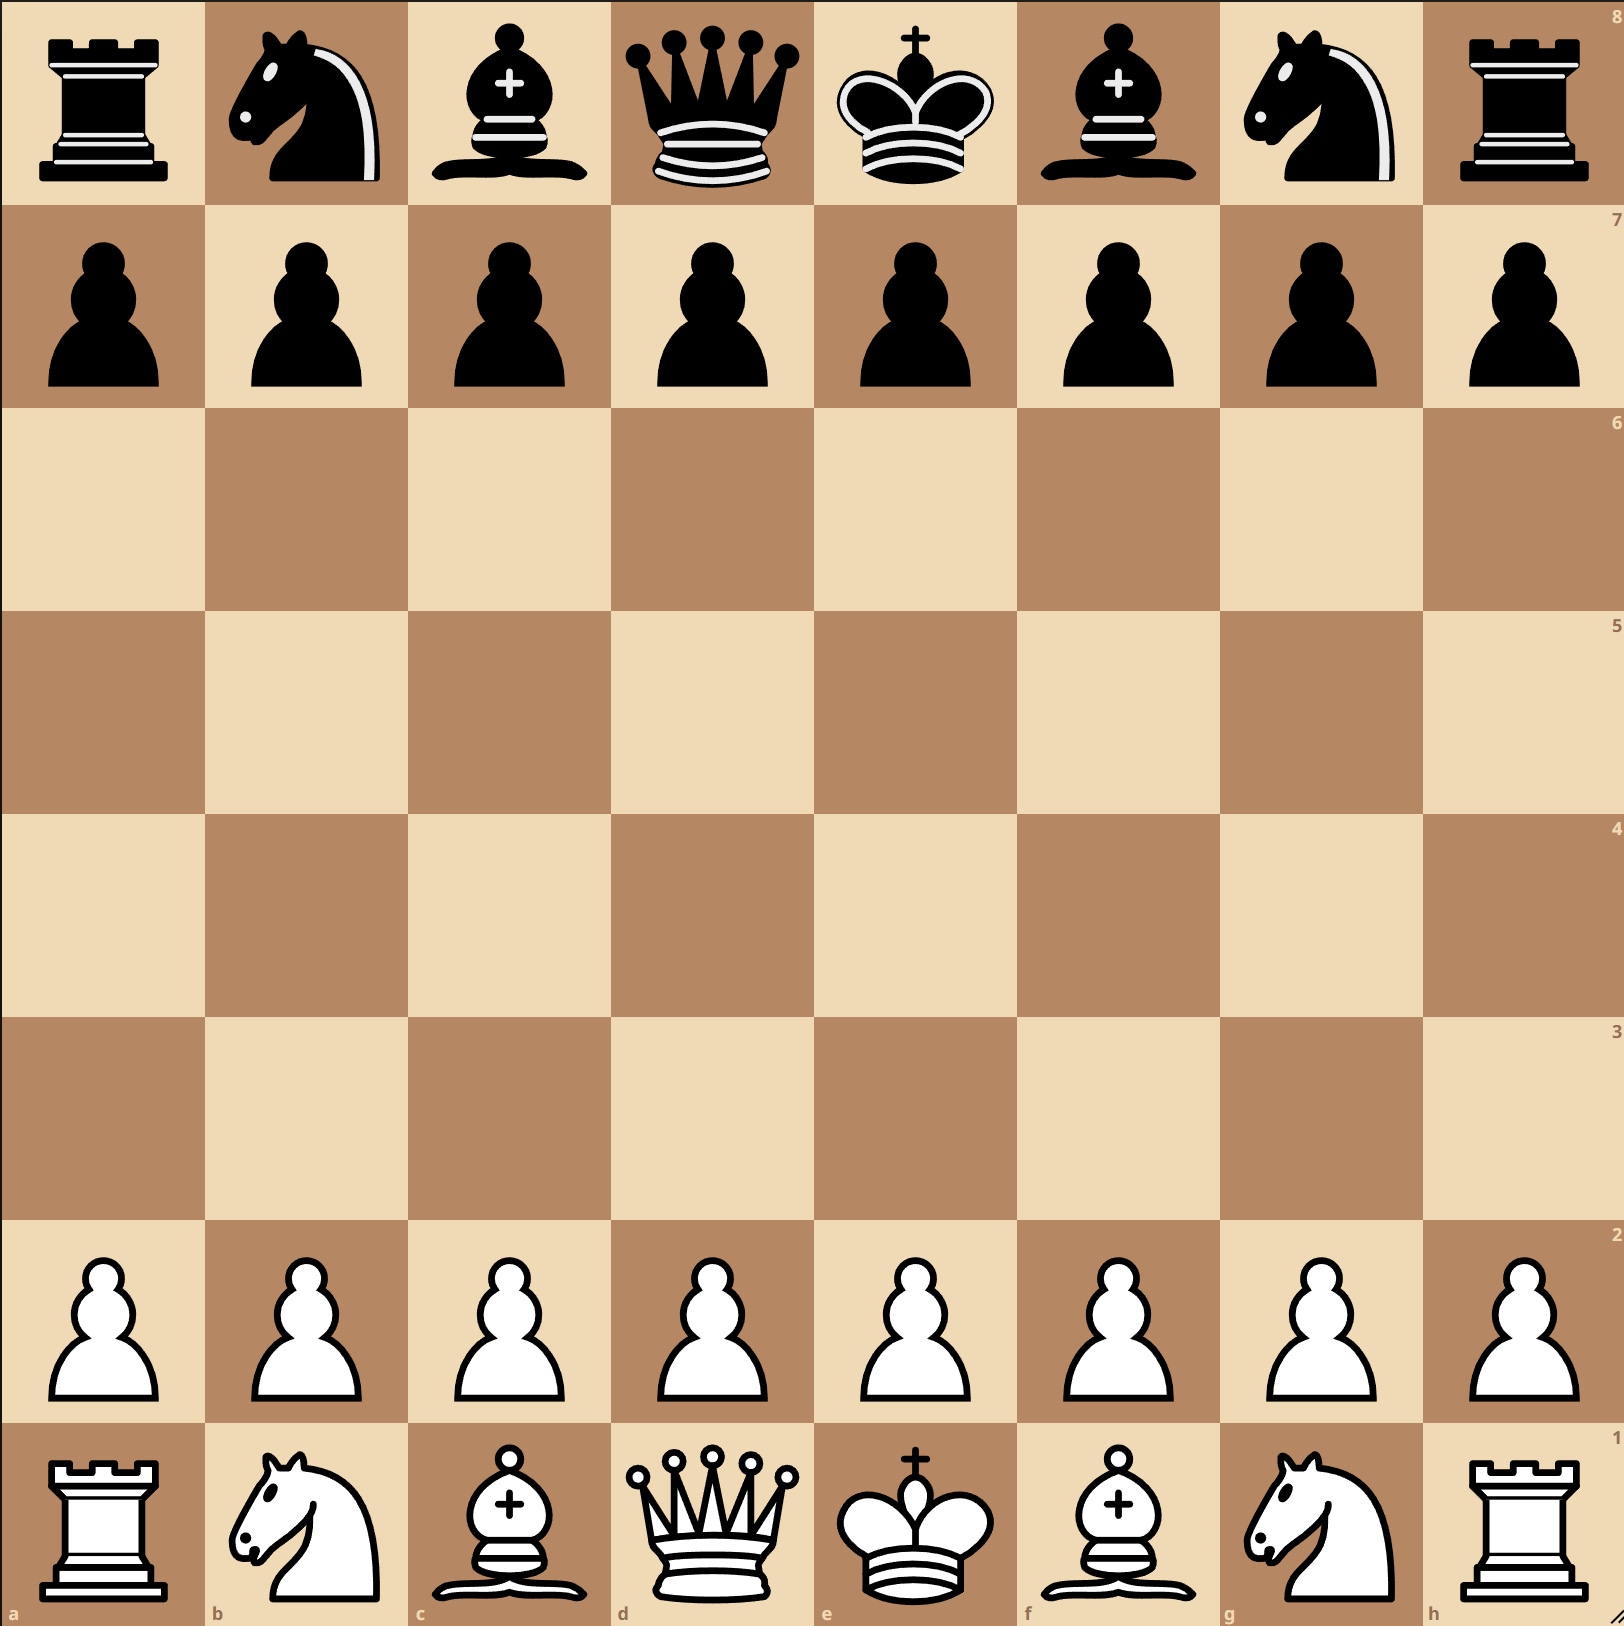
\includegraphics[width=\linewidth/2] {scacchiera.png}
    \caption{Scacchiera nella posizione iniziale di gioco }
\end{figure}

Una bitboard tipica è quella che ci permette di sapere in quali caselle è presente un pedone
nero,per costruirla, operando casella per casella, ci poniamo una domanda "in questa casella
è presente un pedone nero?" se si allora quella casella viene marcata con un 1 , altrimenti viene
marcata con uno 0, il risultato di questa traduzione diventa in questo caso:
\begin{figure}[h!]
    \centering
    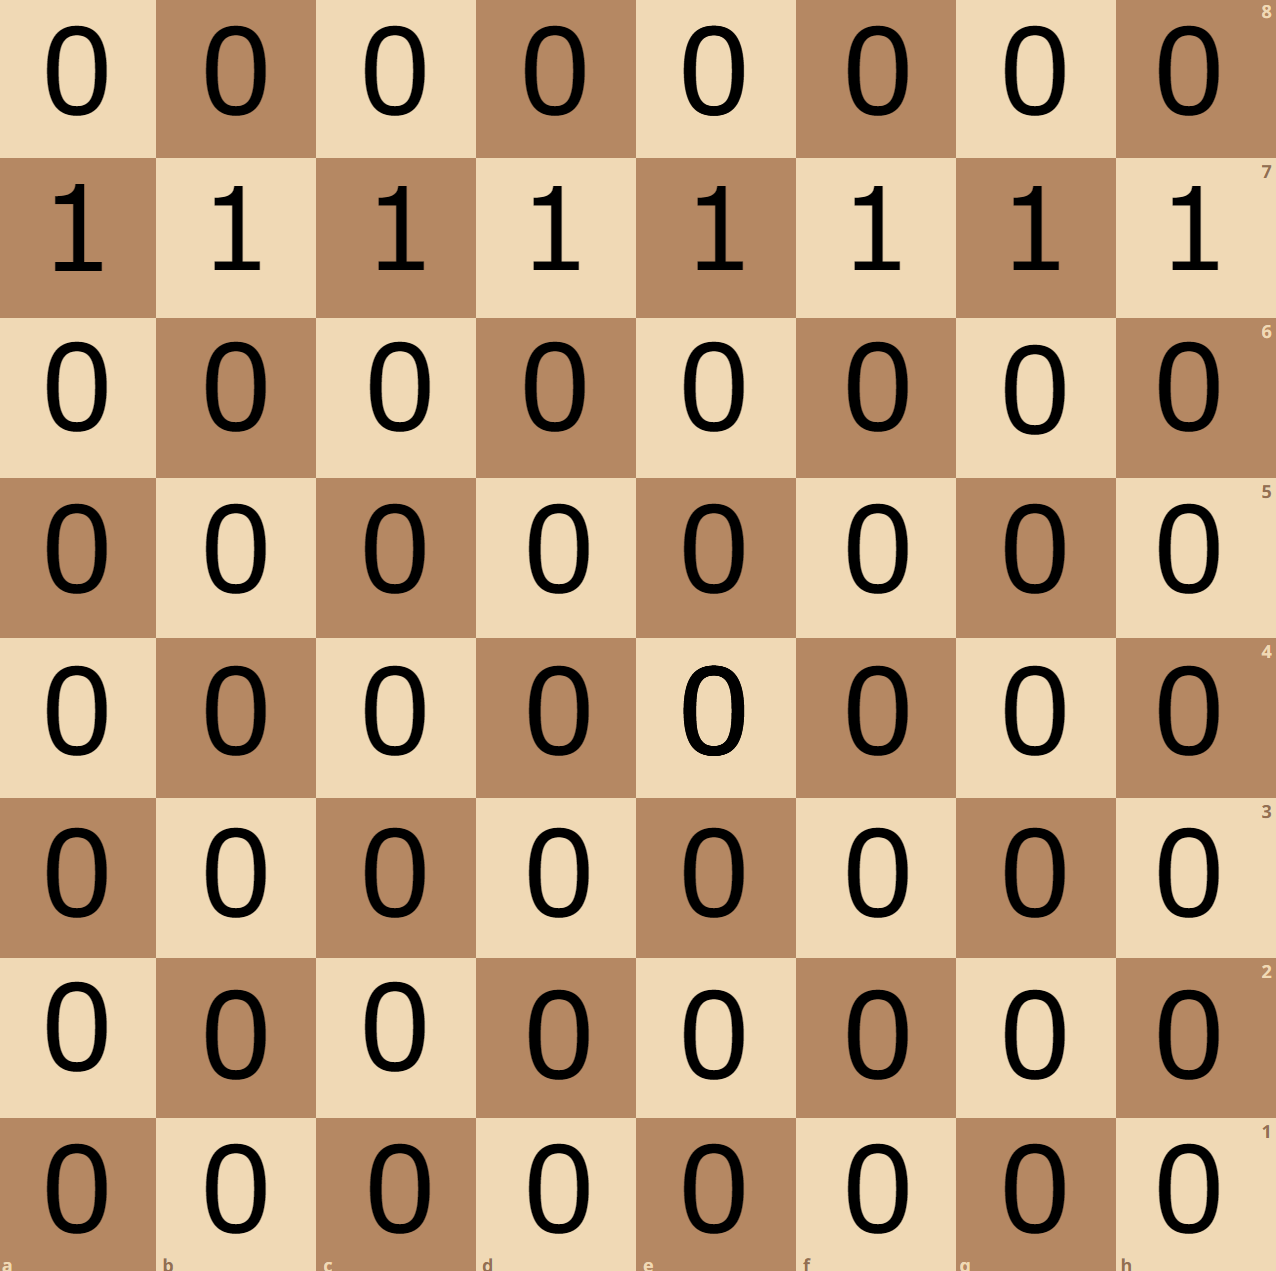
\includegraphics[width=\linewidth/2] {bitboard.png}
    \caption{bitboard}
\end{figure}
La bitboard che codifica questa informazione sarà quindi la parola di 64 bit 00000000 11111111 00000000 00000000 00000000
00000000 00000000 00000000
\subsubsection{Piece-Sets}
rappresentazione con set con un bit per ogni pezzo dentro una parola a 32 bit o 2 parole a 16 bit per ogni lato.
i Piece-sets hanno  delle somiglianze con le bitboards, ma ogni  bit del set non è   direttamente correlato ad una casella,
ma ad un indice  dentro ad una  piece-list. Spesso la bit-position di un  piece-set  implica
, di che tipo e colore il pezzo è. - mentre le  bitboards solitamente mantengono set distinti
per pezzi diversi.




\section{Rappresentazione della scacchiera Casellocentrica}
La rappresentazione casellocentrica  mantiene un associazione inversa rispetto a quella pezzocentrica,
per ogni casella conserviamo in memoria se è vuota o occupata da un pezzo in particolare.
La macro-categoria di  rappresentazione più comune è la Mailbox:

\subsubsection{Mailbox}
La rappresentazione Mailbox è una rappresentazione casellocentrica dove la codifica di ogni casella risiede in una struttura dati
che permette l'accesso casuale ,solitamente si utilizza un array con l'indice che codifica dal numero della casella in array monodimensionali
o dalla coppia traversa/colonna\footnote{termini scacchistici per indicare le righe e le colonne della scacchiera} in array bidimensionali.
Il nome deriva dall'associazione di ogni indice al concetto di "indirizzo" di una casella postale.Le implementazioni più famose e
comuni del concetto di Mailbox sono la 8x8 Board e la 10x12 Board.

\subsubsection{8x8 Board}
Una board 8x8,figura \ref{otto} è una rappresentazione pezzocentrica consistente o in un array bidimensionale di bytes o interi, contenenti rappresentazioni codificate
per i pezzi e per la casella vuota, con i due indici ricavati dalla coppia traversa/colonna che identifica la casella sulla scacchiera ,
o più comunemente un array monodimensionale con indici da 0 a 63,uno per ogni casella della scacchiera.
Questo tipo di rappresentazione è usata spesso come rappresentazione ridondante all'interno di programmi che utilizzano bitboards
per individuare se e quali pezzi sono presenti su una casella in maniera efficiente.
\begin{figure}[!ht]
    \centering
    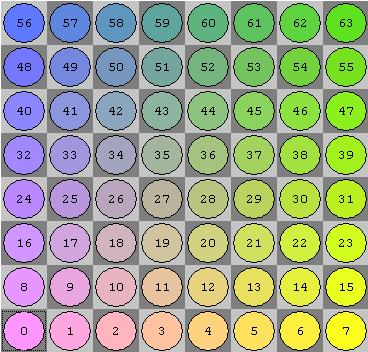
\includegraphics[width=\linewidth/2]{8x8 board.png}
    \caption{board numbering}
    \label{otto}
\end{figure}

\subsubsection{10x12 Board}
Una board 10x12  contorna una  board 8x8   con traverse e colonne sentinelle  per individuare  indici al di fuori della scacchiera durante la generazione delle mosse
\vfill
\begin{figure}[!ht]
    \centering
    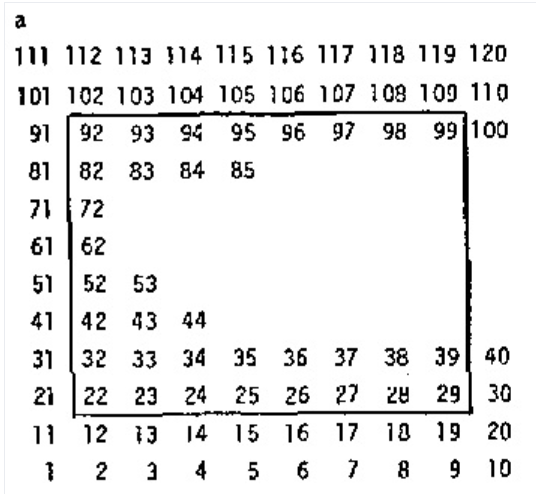
\includegraphics[width=\linewidth/2]{10x12 board.png}
    \caption{Rappresentazione di una board 10x12,notare come le 2 traverse extra sopra e sotto siano necessarie per evitare accessi out of bounds in caso di cavalli posizionati sulla prima o ottava fila }
\end{figure}
\vfill
\clearpage


\section{Rappresentazione dei pezzi}
una volta scelto il tipo di rappresentazione della scacchiera si può iniziare a pensare alla rappresentazione dei pezzi,
anche se può sembrare controintuitivo i pezzi non hanno bisogno di una struttura elaborata,la generazione delle possibili
mosse verrà gestita nella move generation ed il loro spostamento all'interno della scacchiera verrà gestito dalla funzione
MakeMove (approfondimenti riguardo questi due argomenti sono presenti nel capitolo \ref{move generation}  ),per i pezzi quindi abbiamo bisogno di una
rappresentazione semplice, di facile interpretazione e che occupi poco spazio.\\Rappresentazioni molto comuni sono quella
tramite interi, dove ad ogni tipo di pezzo viene assegnato un numero che funge da identificativo univoco e quella tramite
caratteri, dove ad ogni tipo di pezzo viene assegnato un carattere che lo identifica.


